\section{Results and Discussion}
For this lab course, a \ce{ZnO} thin film was grown on a c-sapphire substrate using 
a \ac{pld} chamber. 
The thin film was deposited at a pressure of \qty{0.002}{\milli\bar} with \num{300}
pulses at \qty{1}{\hertz} and \num{10000} subsequent pulses at \qty{15}{\hertz}.
A \ce{KrF} excimer laser with a pulse energy of \qty{650}{\milli\joule} was used. 
During deposition and for \qty{5}{\minute} afterward, the substrate was heated 
using a resistive heater to about \qty{700}{\degreeCelsius}.

After deposition, the \ce{ZnO} sample as well as a \ce{SrTiO3} thin film were 
investigated using a \ac{rheed} setup.
The obtained diffraction pattern for different azimuthal angles are shown in 
\cref{fig:rheed1} and \cref{fig:rheed2}.

The \ce{SrTiO3} diffraction pattern at \qtylist{0; 90; 180; 270}{\degree} 
as well as the pattern at \qtylist{45; 135; 225; 315}{\degree} in \cref{fig:rheed1} are 
identical. 
These are equal if the reciprocal lattice is transformed into itself by rotation.
Therefore, the surface lattice has a four-fold symmetry, indicating a
cubic surface lattice structure. 

The \ce{ZnO} thin shows identical patterns at \qtylist{0;60;120;180;240;300}{\degree} 
as well as at \qtylist{30;90;150;210;270;330}{\degree} in \cref{fig:rheed2}.
This indicates a six-fold symmetry of the surface lattice, which is typical for
hexagonal lattices.

Both samples show two distinct diffraction patterns with a \qty{45}{\degree} or 
\qty{30}{\degree} angles between them.
This is reasonable, as diffraction patterns only occur for Laue planes that are 
parallel to the surface and contain sufficient atoms.
For both \ce{SrTiO3} and \ce{ZnO}, the observed Laue planes are $(10)$ and $(11)$,
see \cref{fig:planes}.

 \newpage
\begin{figure*}
    \centering
    % first block
    \begin{subfigure}{0.2\linewidth}
        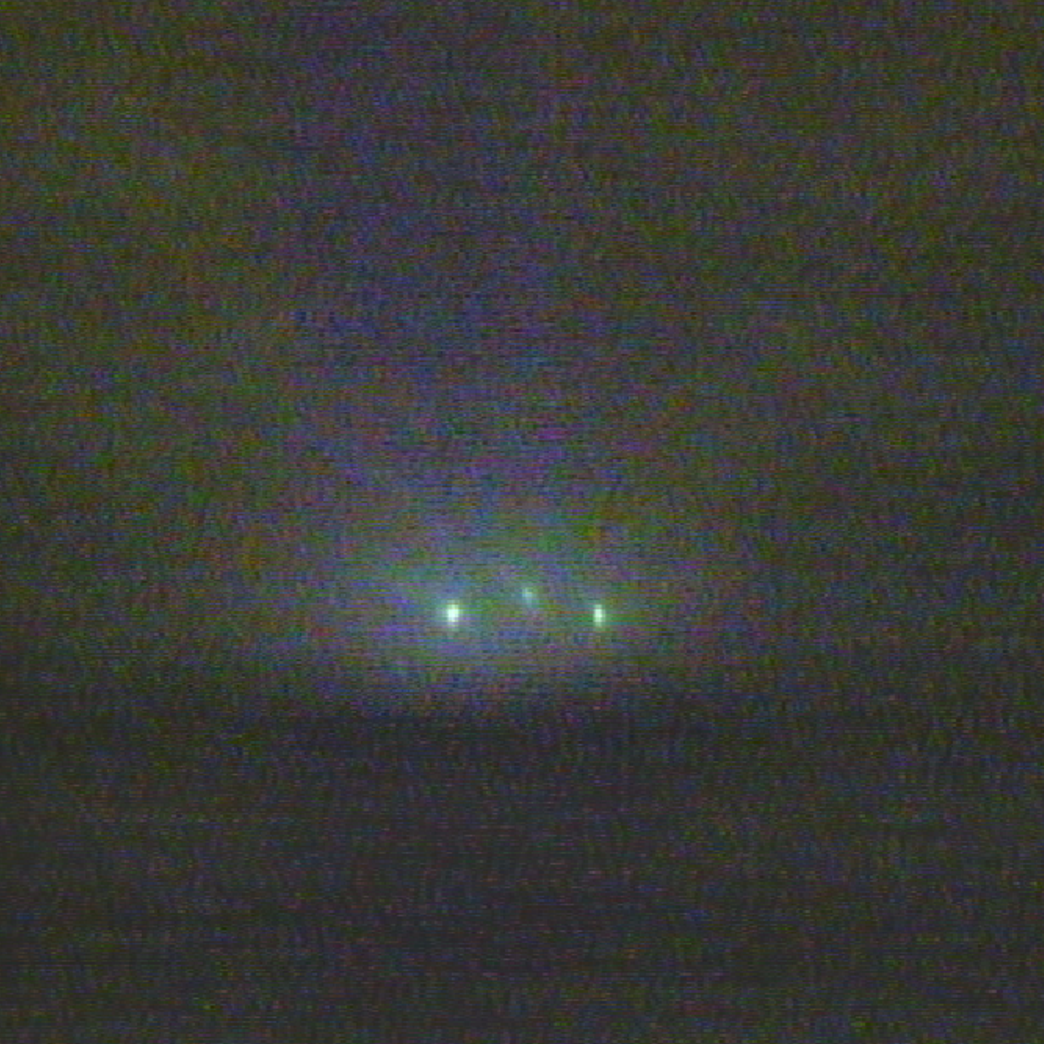
\includegraphics[width=\textwidth]{../data/edited/1_1_7deg.pdf}
        \caption{\qty{0}{\degree}}
    \end{subfigure}
    \begin{subfigure}{0.2\linewidth}
        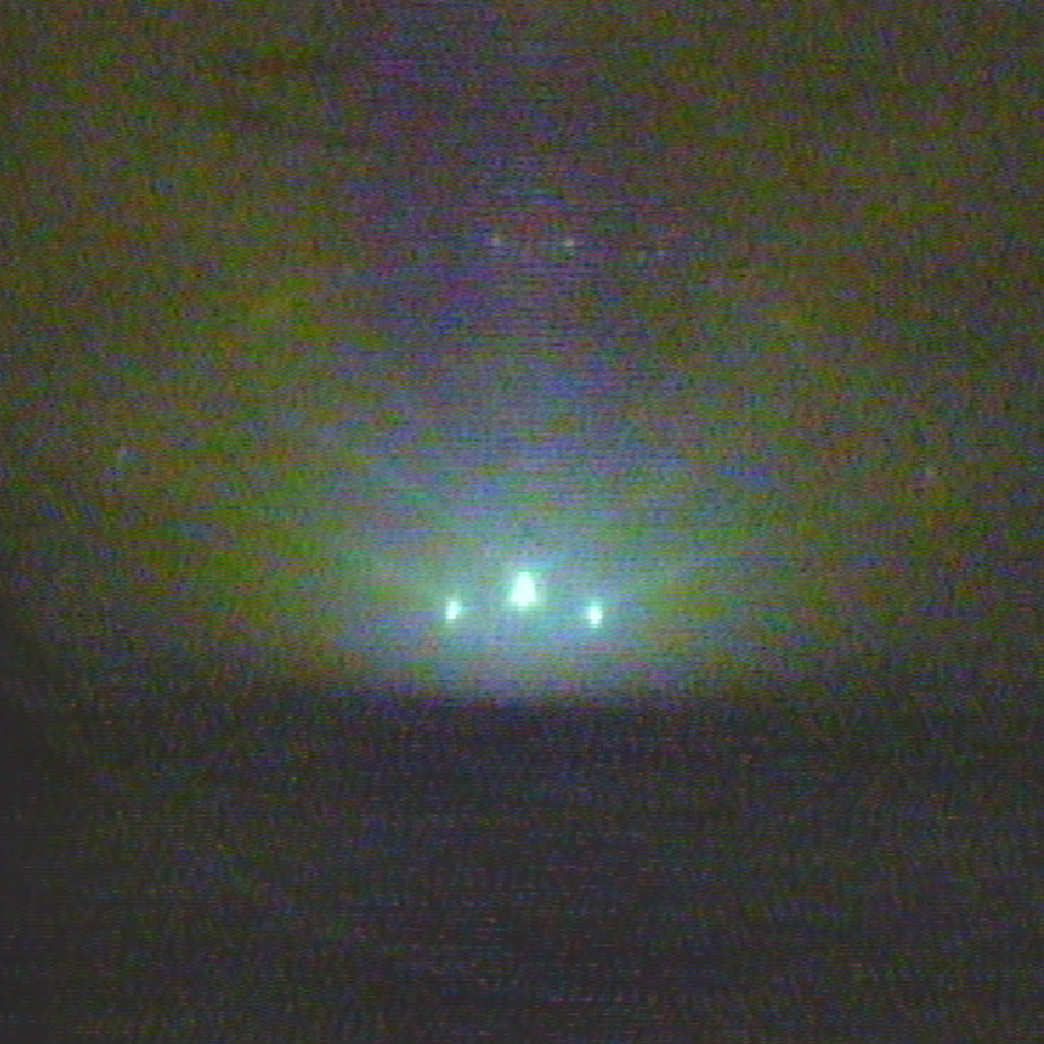
\includegraphics[width=\textwidth]{../data/edited/1_1_97deg.pdf}
        \caption{\qty{90}{\degree}}
    \end{subfigure}
    \begin{subfigure}{0.2\linewidth}
        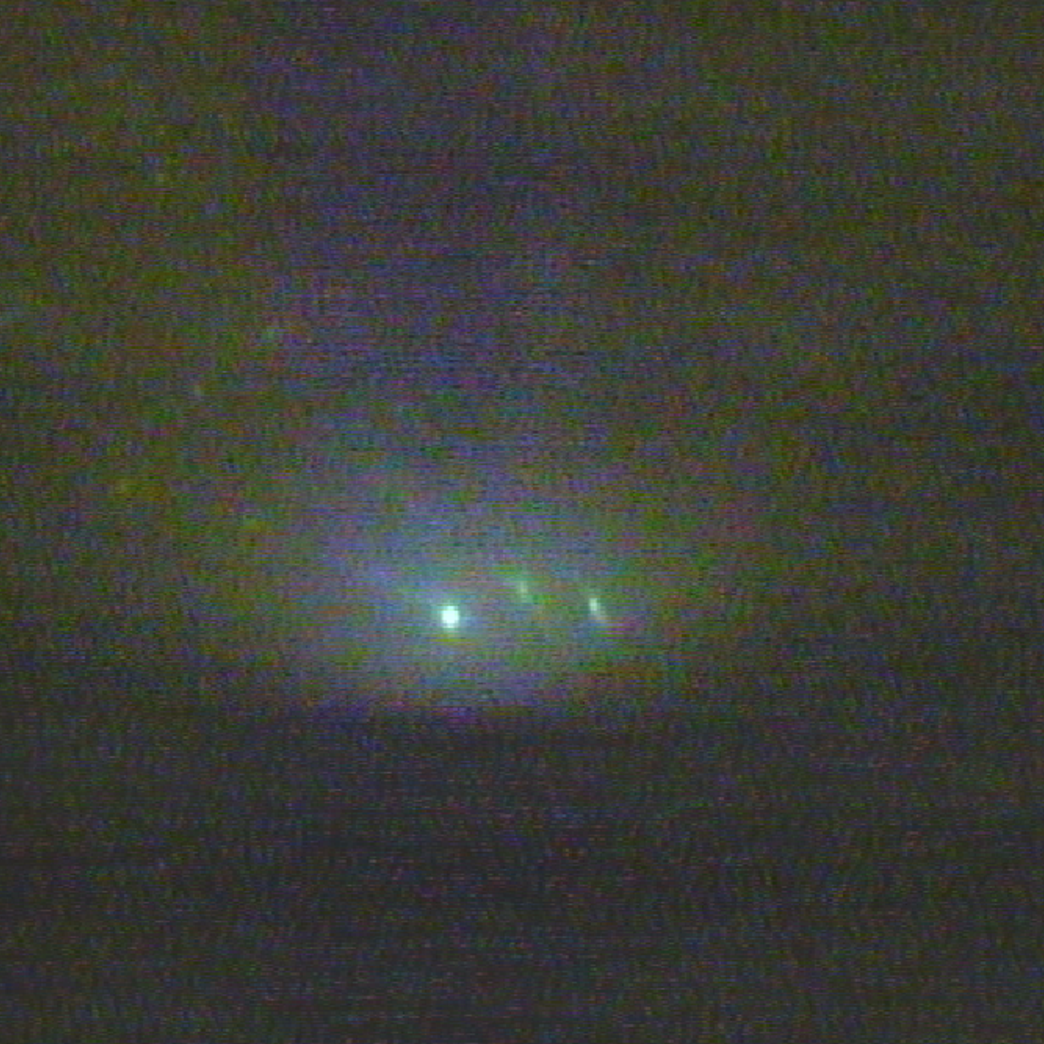
\includegraphics[width=\textwidth]{../data/edited/1_1_187deg.pdf}
        \caption{\qty{180}{\degree}}
    \end{subfigure}
    \begin{subfigure}{0.2\linewidth}
        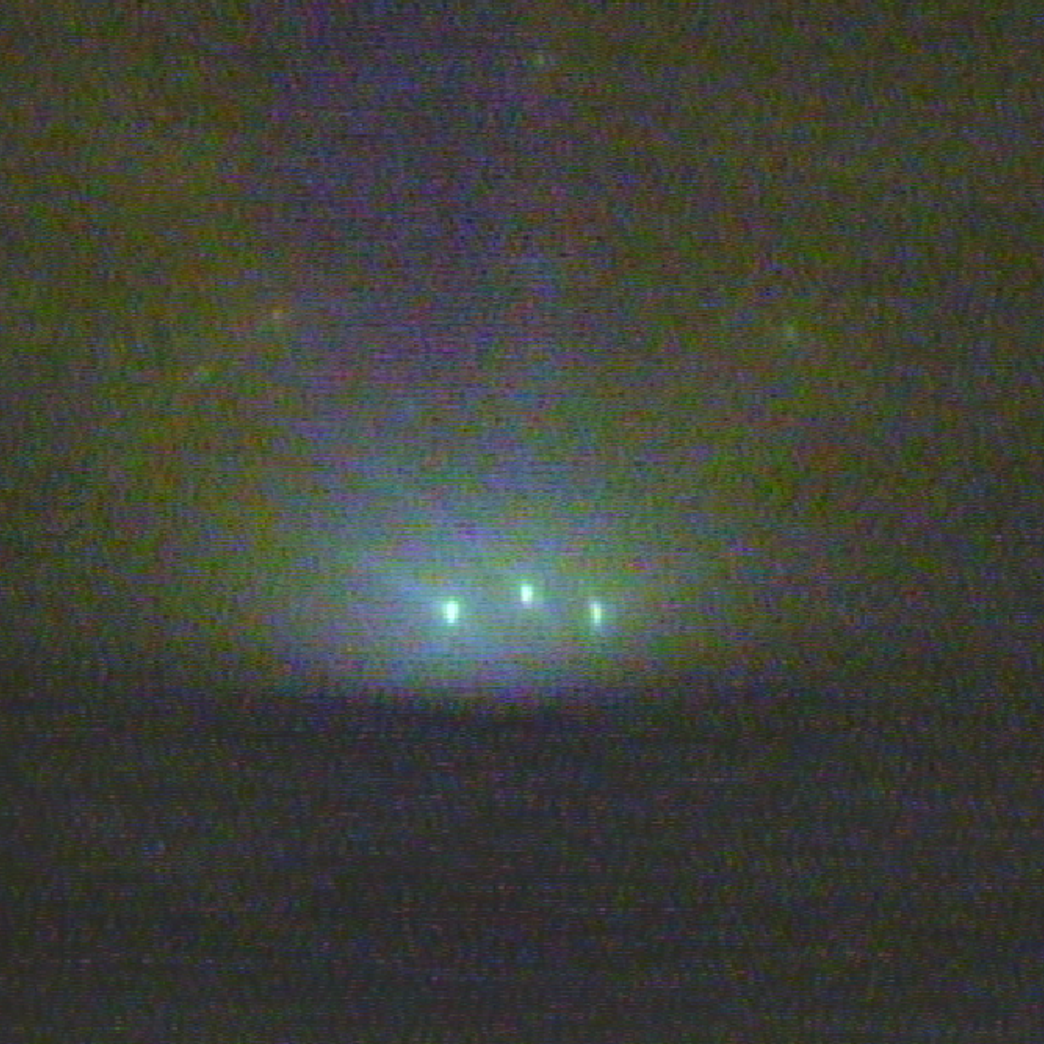
\includegraphics[width=\textwidth]{../data/edited/1_1_277deg.pdf}
        \caption{\qty{270}{\degree}}
    \end{subfigure}

    % second block
    \begin{subfigure}{0.2\linewidth}
        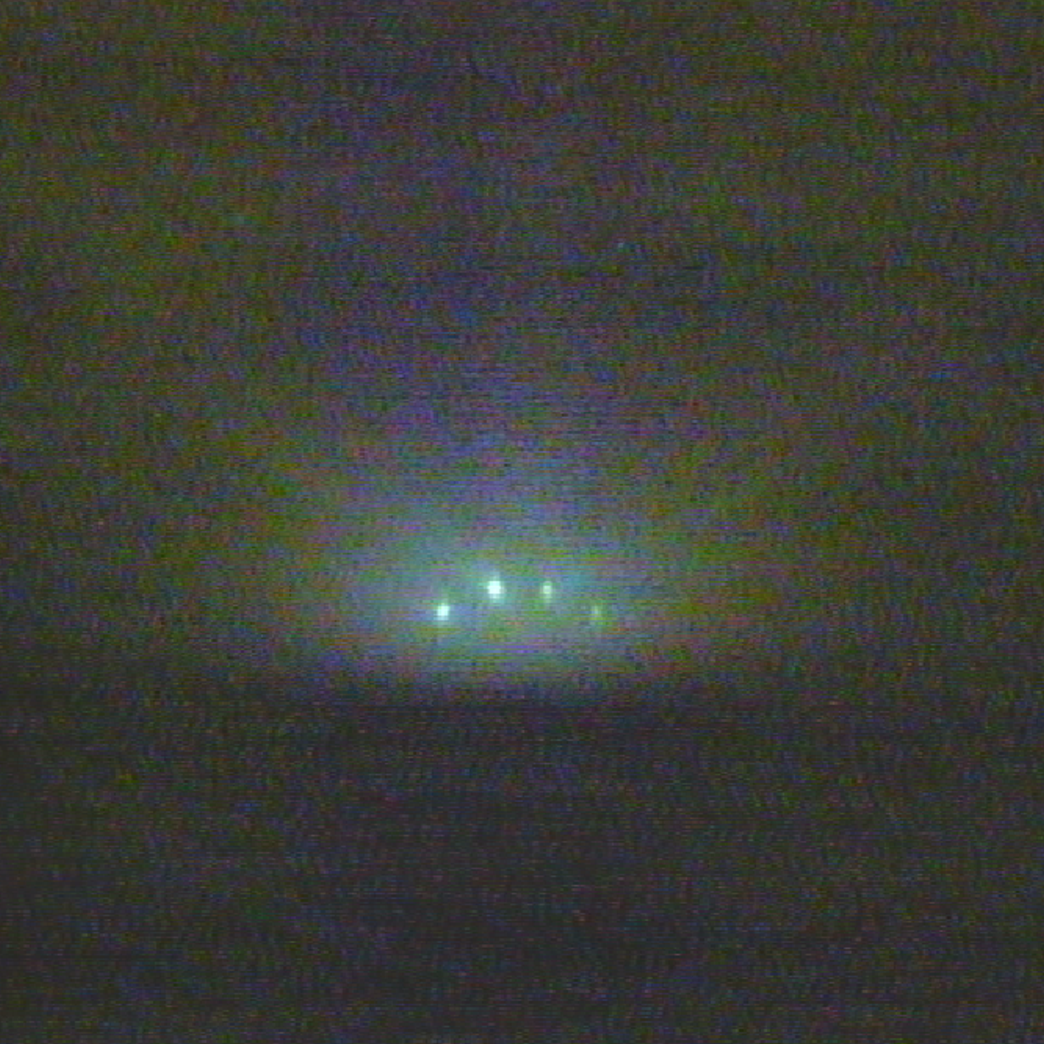
\includegraphics[width=\textwidth]{../data/edited/1_2_52deg.pdf}
        \caption{\qty{45}{\degree}}
    \end{subfigure}
    \begin{subfigure}{0.2\linewidth}
        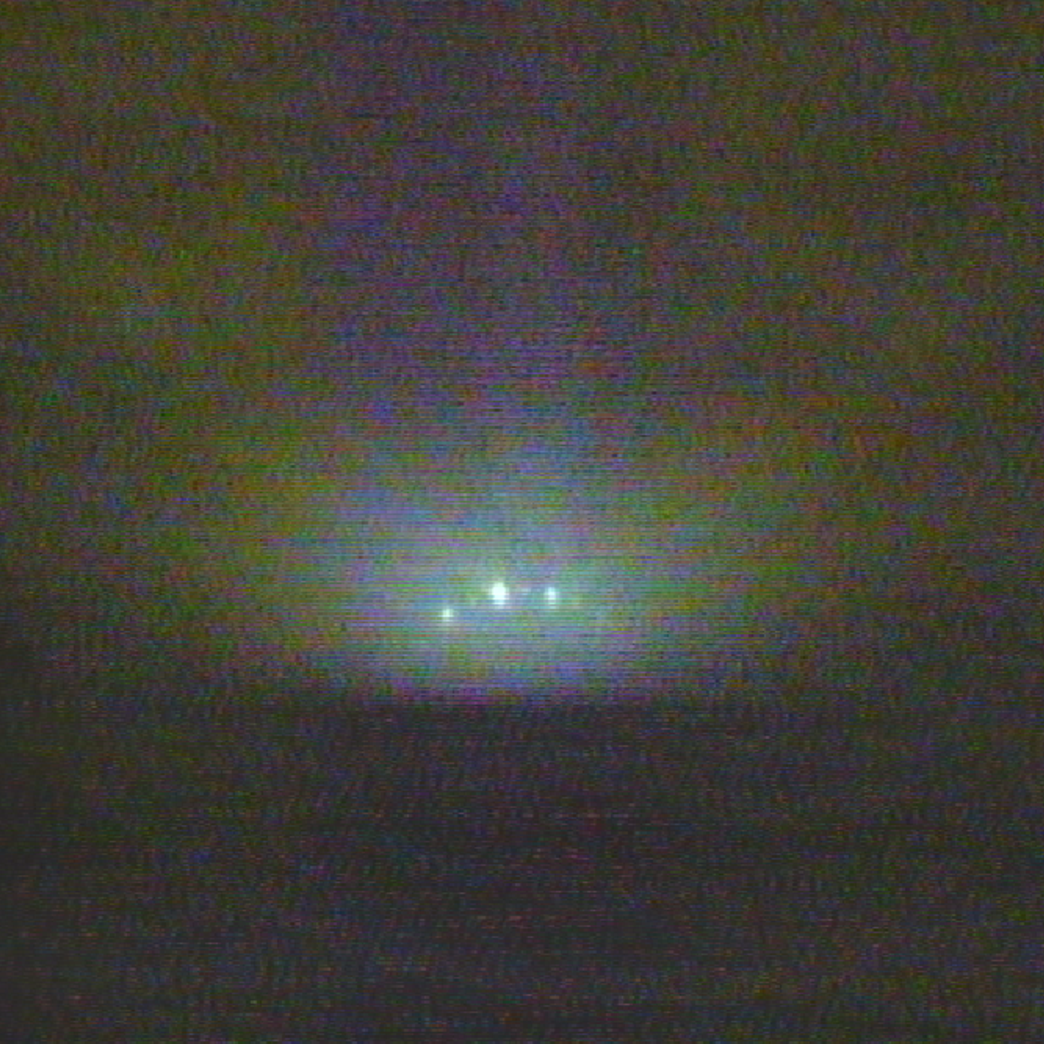
\includegraphics[width=\textwidth]{../data/edited/1_2_142deg.pdf}
        \caption{\qty{135}{\degree}}
    \end{subfigure}
    \begin{subfigure}{0.2\linewidth}
        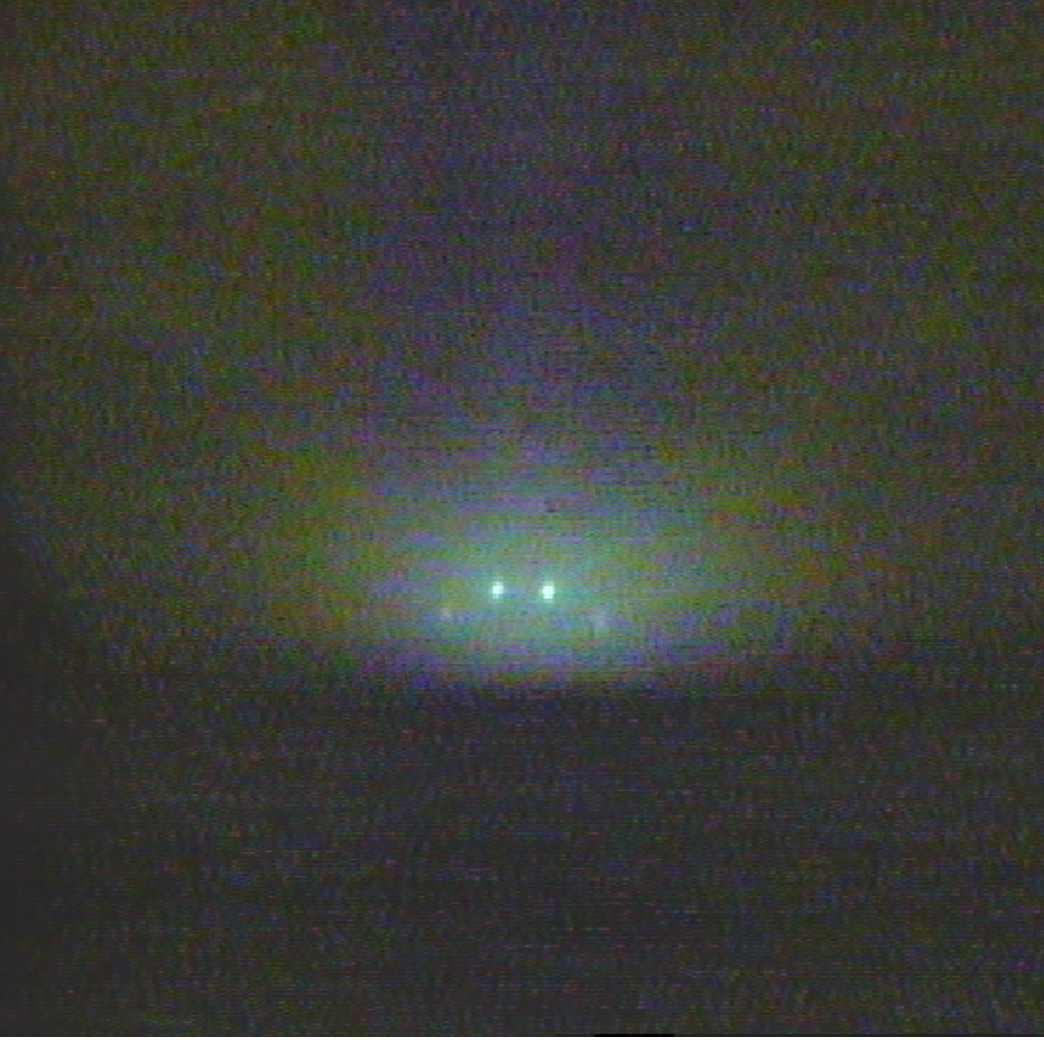
\includegraphics[width=\textwidth]{../data/edited/1_2_232deg.pdf}
        \caption{\qty{225}{\degree}}
    \end{subfigure}
    \begin{subfigure}{0.2\linewidth}
        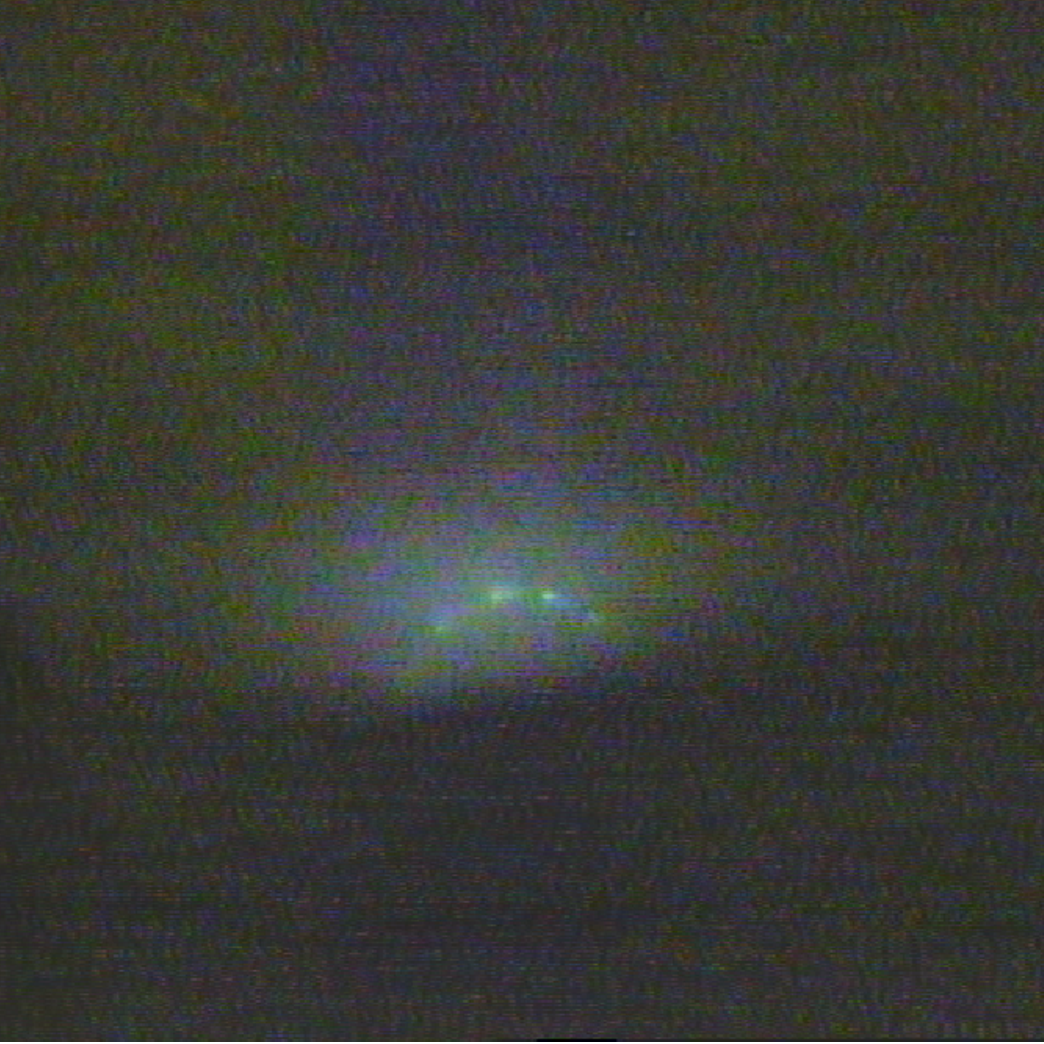
\includegraphics[width=\textwidth]{../data/edited/1_2_322deg.pdf}
        \caption{\qty{315}{\degree}}
    \end{subfigure}

    \caption{\ac{rheed} patterns of the \ce{SrTiO3} thin film for different azimuthal 
    angles.}
    \label{fig:rheed1}
\end{figure*}

\begin{figure*}
    \centering
    % fist block
    \begin{subfigure}{0.2\linewidth}
        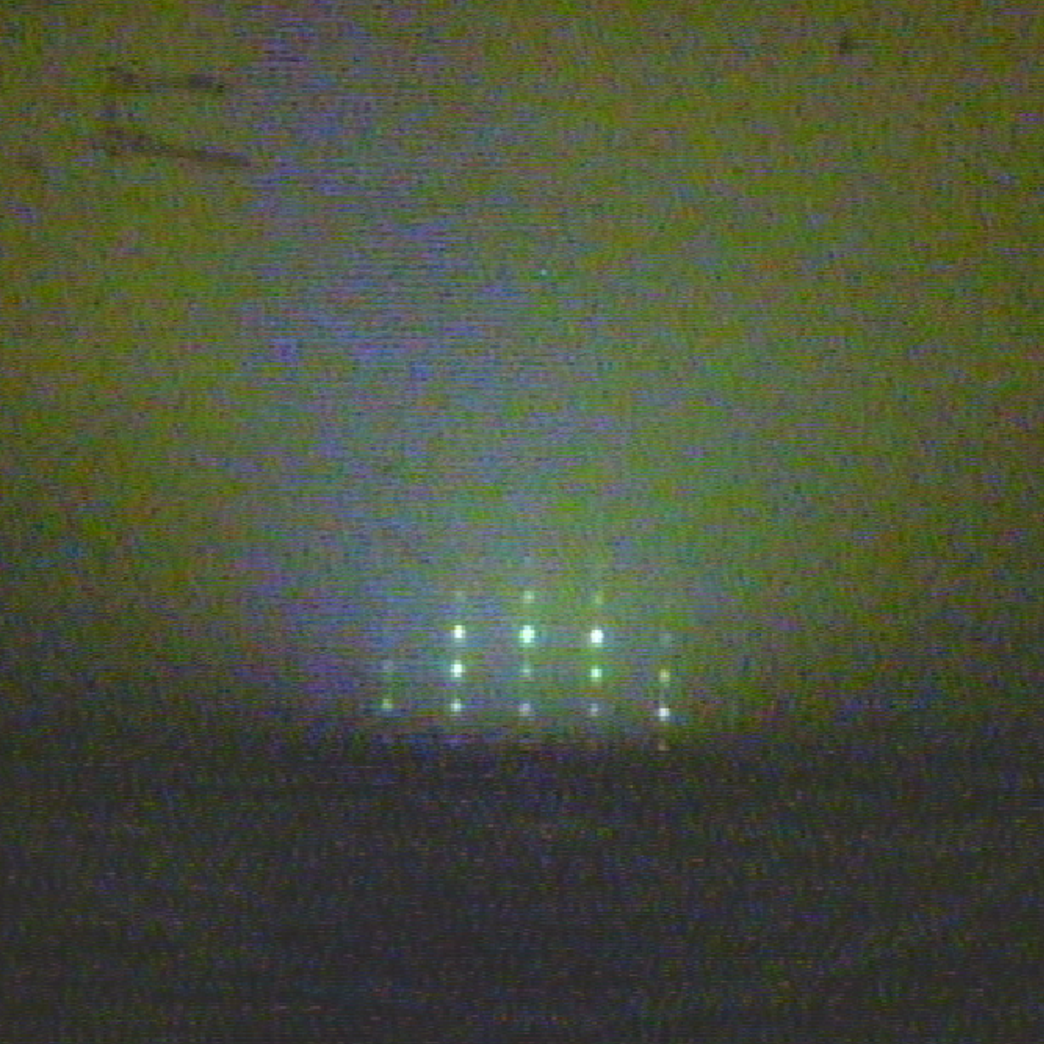
\includegraphics[width=\textwidth]{../data/edited/2_1_23deg.pdf}
        \caption{\qty{0}{\degree}}
    \end{subfigure}
    \begin{subfigure}{0.2\linewidth}
        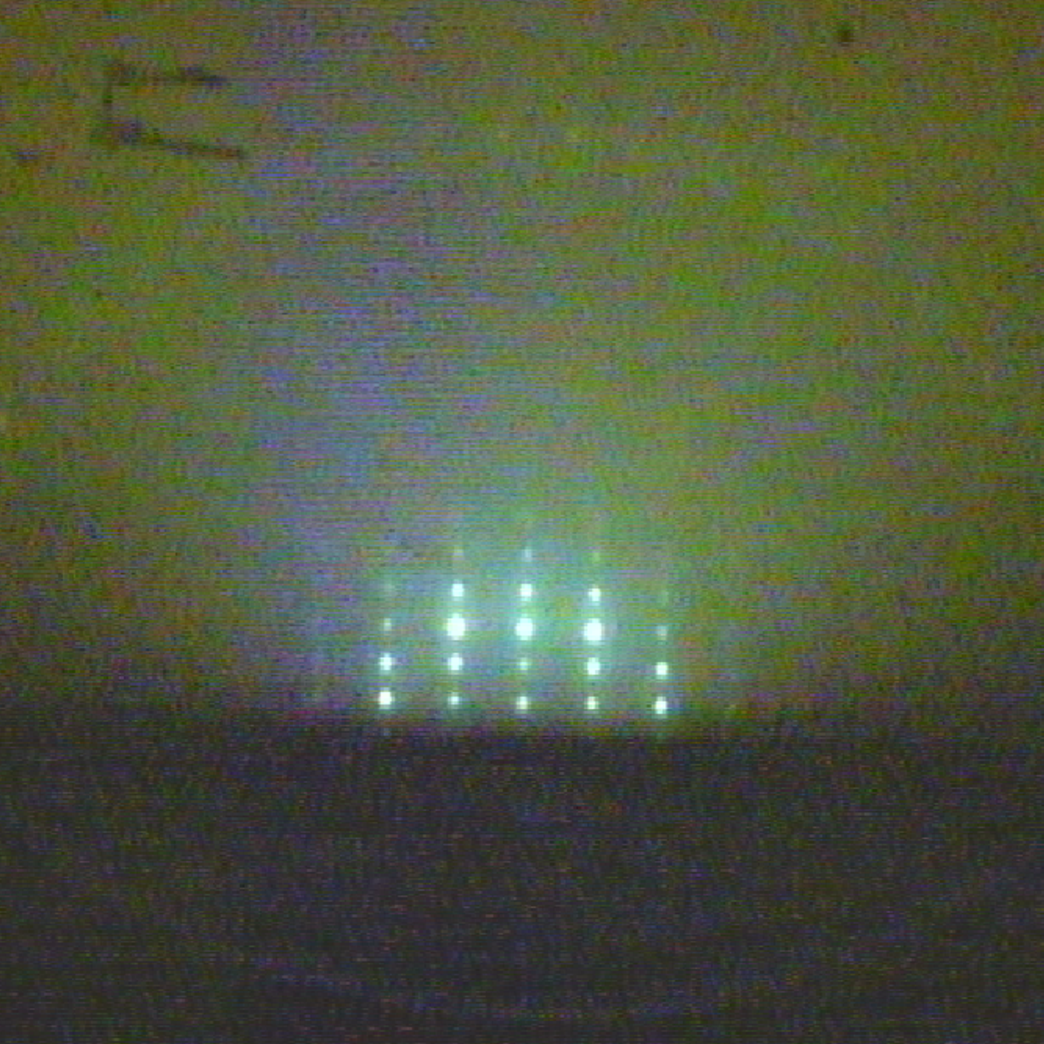
\includegraphics[width=\textwidth]{../data/edited/2_1_83deg.pdf}
        \caption{\qty{60}{\degree}}
    \end{subfigure}
    \begin{subfigure}{0.2\linewidth}
        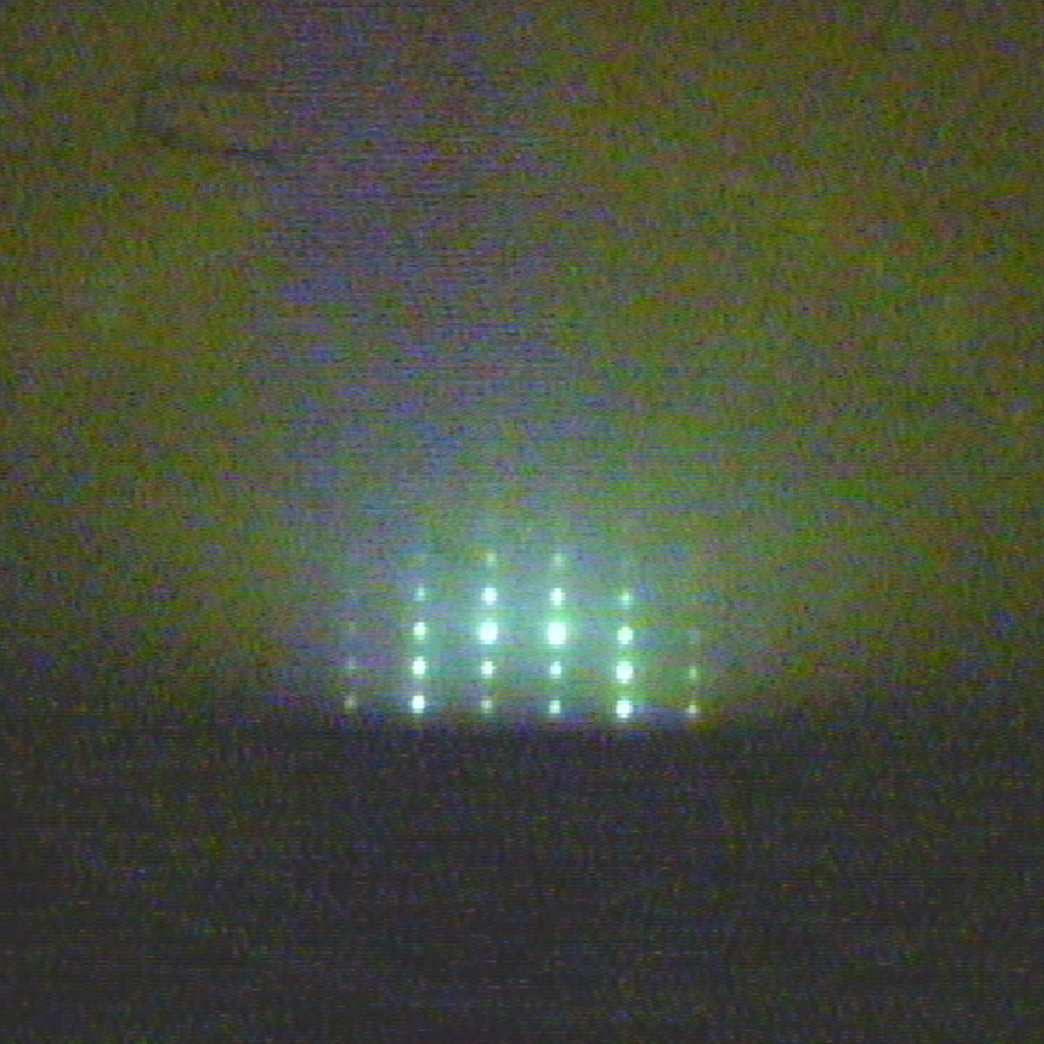
\includegraphics[width=\textwidth]{../data/edited/2_1_143deg.pdf}
        \caption{\qty{120}{\degree}}
    \end{subfigure}
    \begin{subfigure}{0.2\linewidth}
        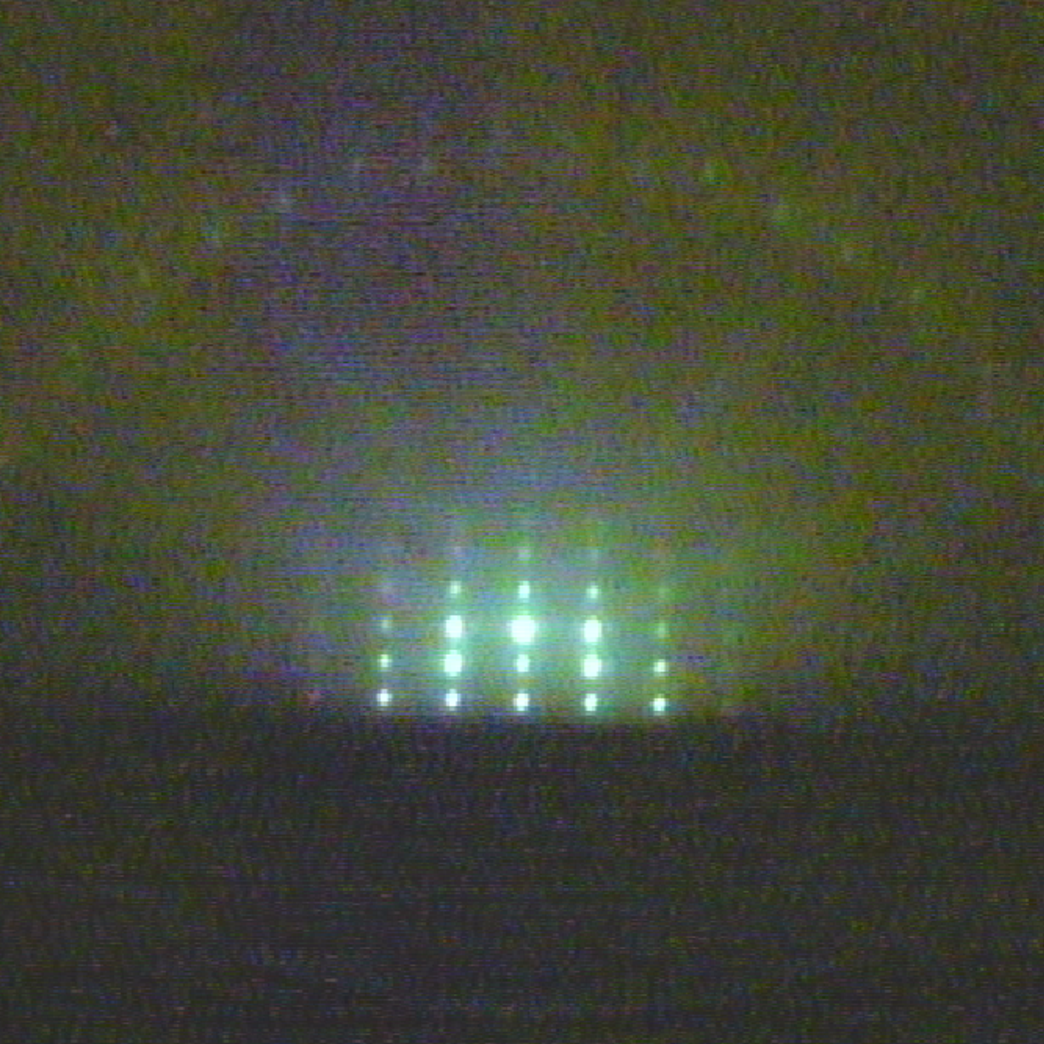
\includegraphics[width=\textwidth]{../data/edited/2_1_203deg.pdf}
        \caption{\qty{180}{\degree}}
    \end{subfigure}
    \begin{subfigure}{0.2\linewidth}
        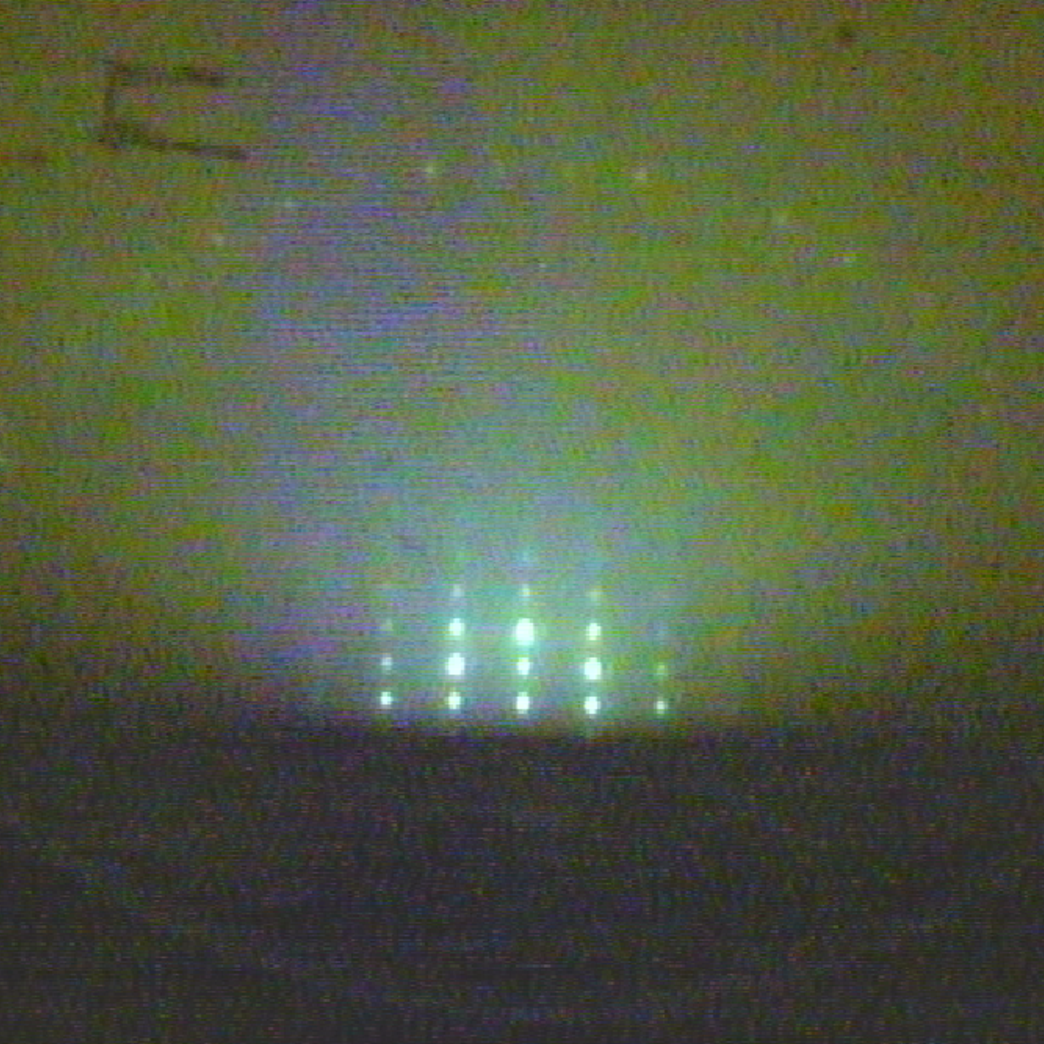
\includegraphics[width=\textwidth]{../data/edited/2_1_263deg.pdf}
        \caption{\qty{240}{\degree}}
    \end{subfigure}
    \begin{subfigure}{0.2\linewidth}
        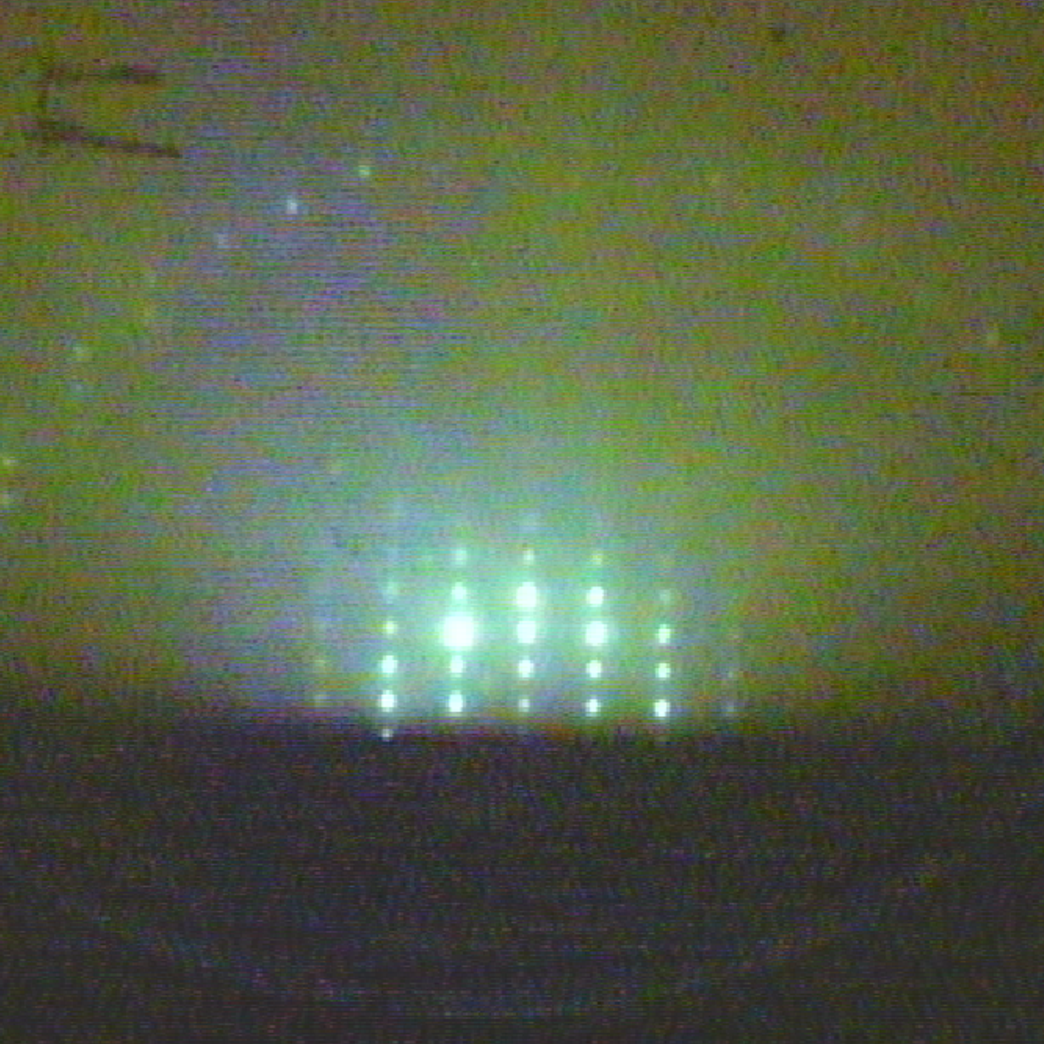
\includegraphics[width=\textwidth]{../data/edited/2_1_323deg.pdf}
        \caption{\qty{300}{\degree}}
    \end{subfigure}
    % second block
    \begin{subfigure}{0.2\linewidth}
        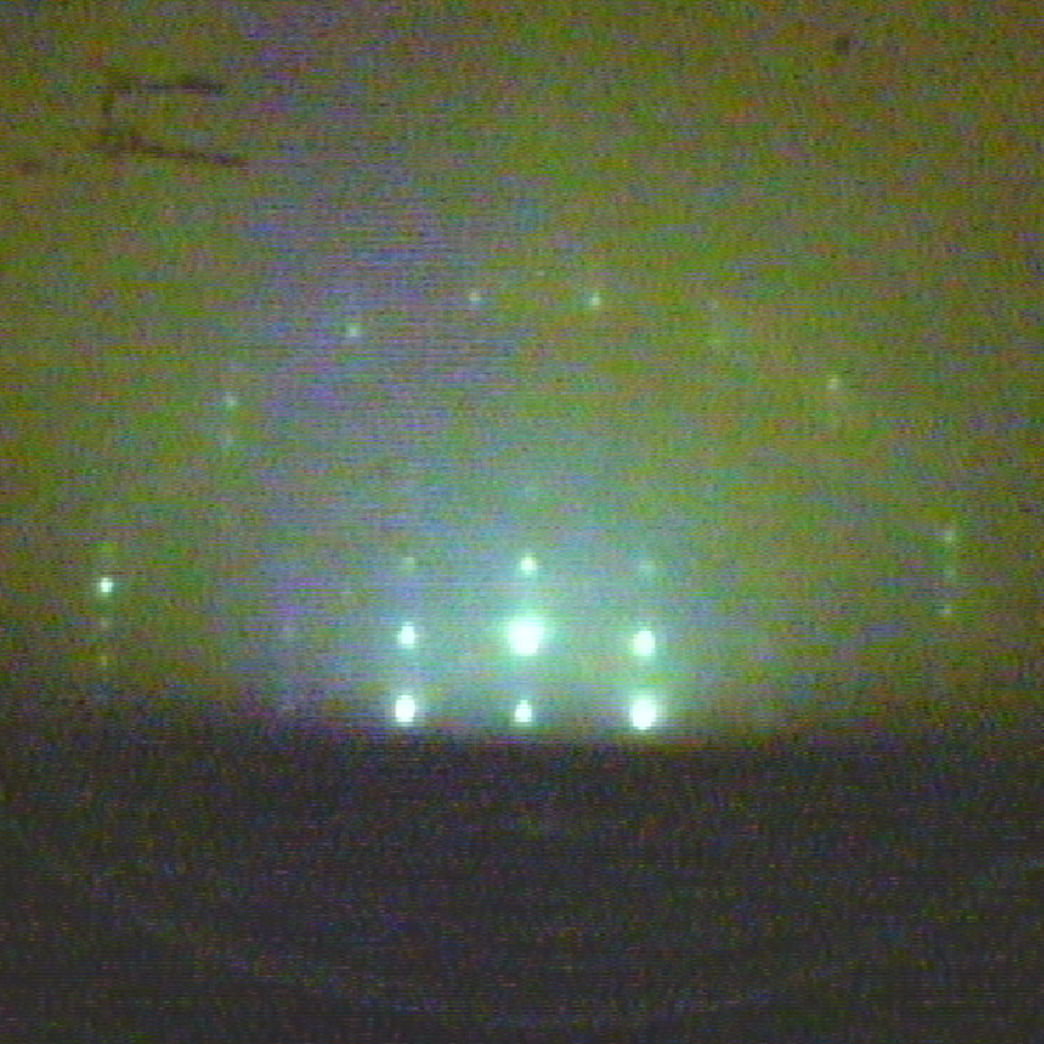
\includegraphics[width=\textwidth]{../data/edited/2_2_53deg.pdf}
        \caption{\qty{30}{\degree}}
    \end{subfigure}
    \begin{subfigure}{0.2\linewidth}
        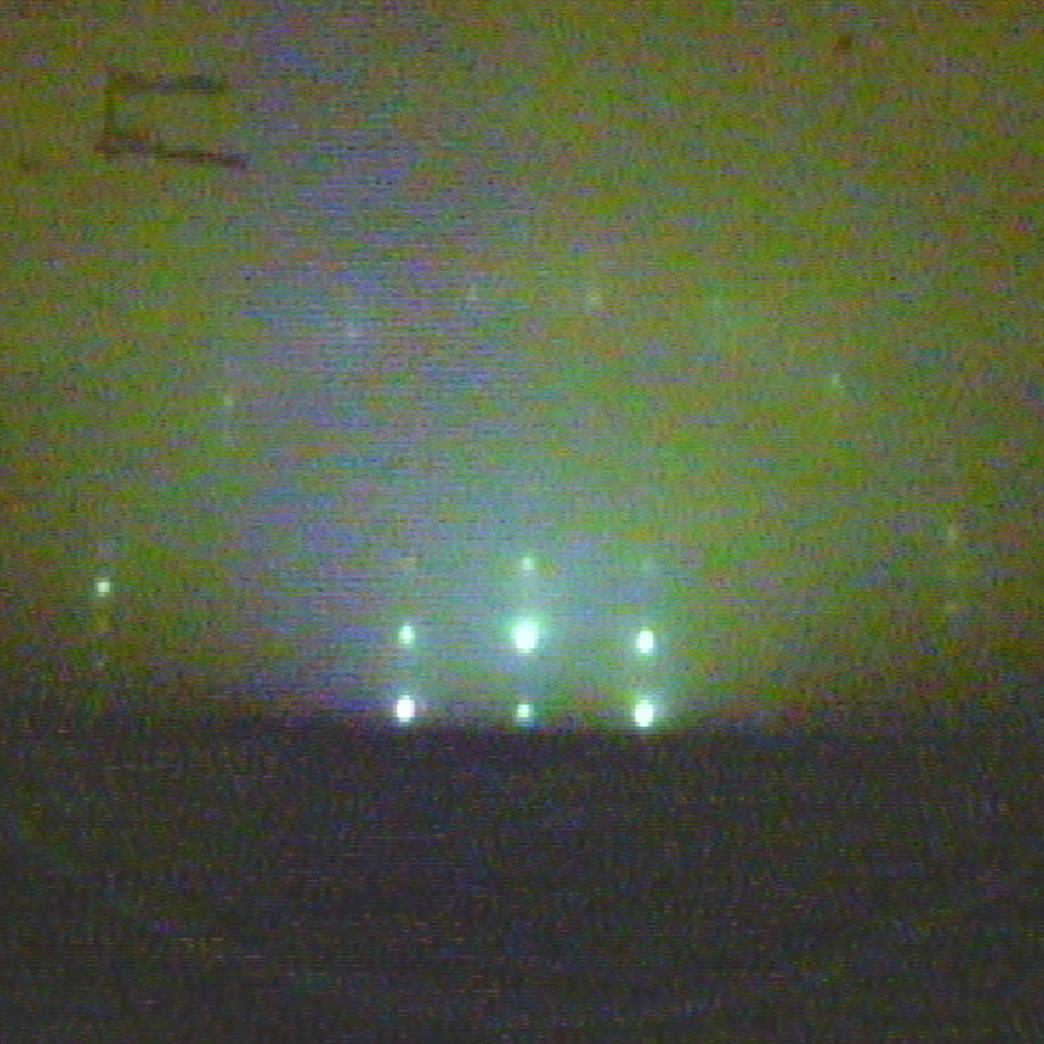
\includegraphics[width=\textwidth]{../data/edited/2_2_113deg.pdf}
        \caption{\qty{90}{\degree}}
    \end{subfigure}
    \begin{subfigure}{0.2\linewidth}
        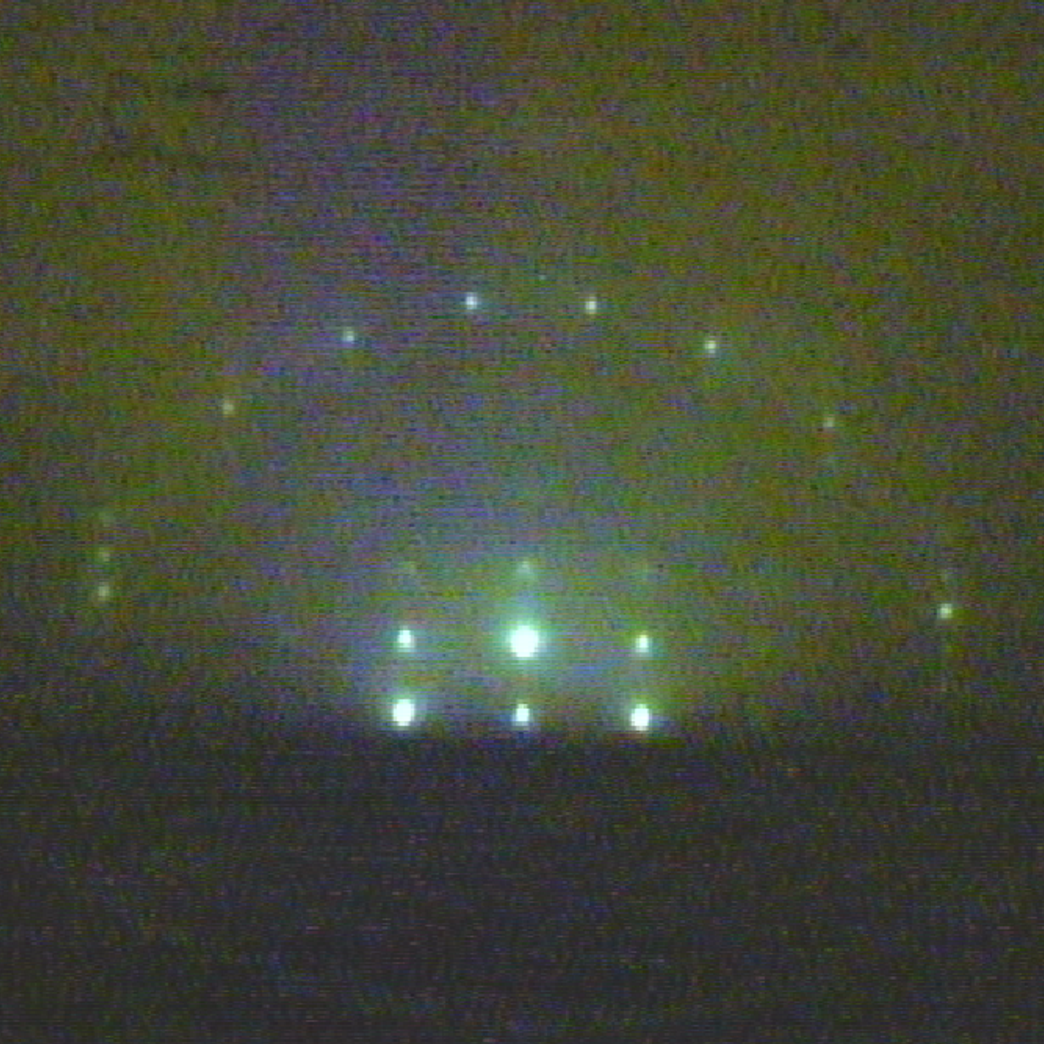
\includegraphics[width=\textwidth]{../data/edited/2_2_173deg.pdf}
        \caption{\qty{150}{\degree}}
    \end{subfigure}
    \begin{subfigure}{0.2\linewidth}
        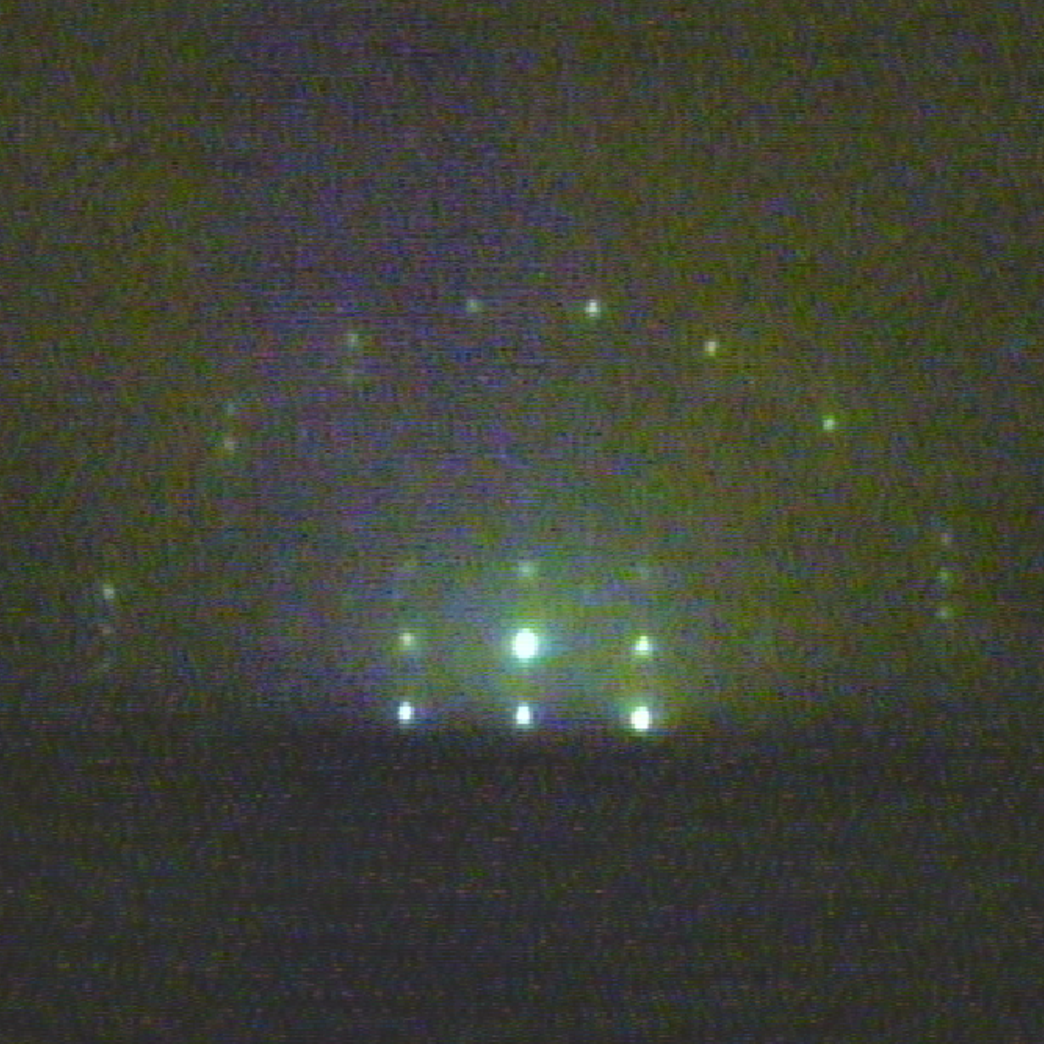
\includegraphics[width=\textwidth]{../data/edited/2_2_233deg.pdf}
        \caption{\qty{210}{\degree}}
    \end{subfigure}
    \begin{subfigure}{0.2\linewidth}
        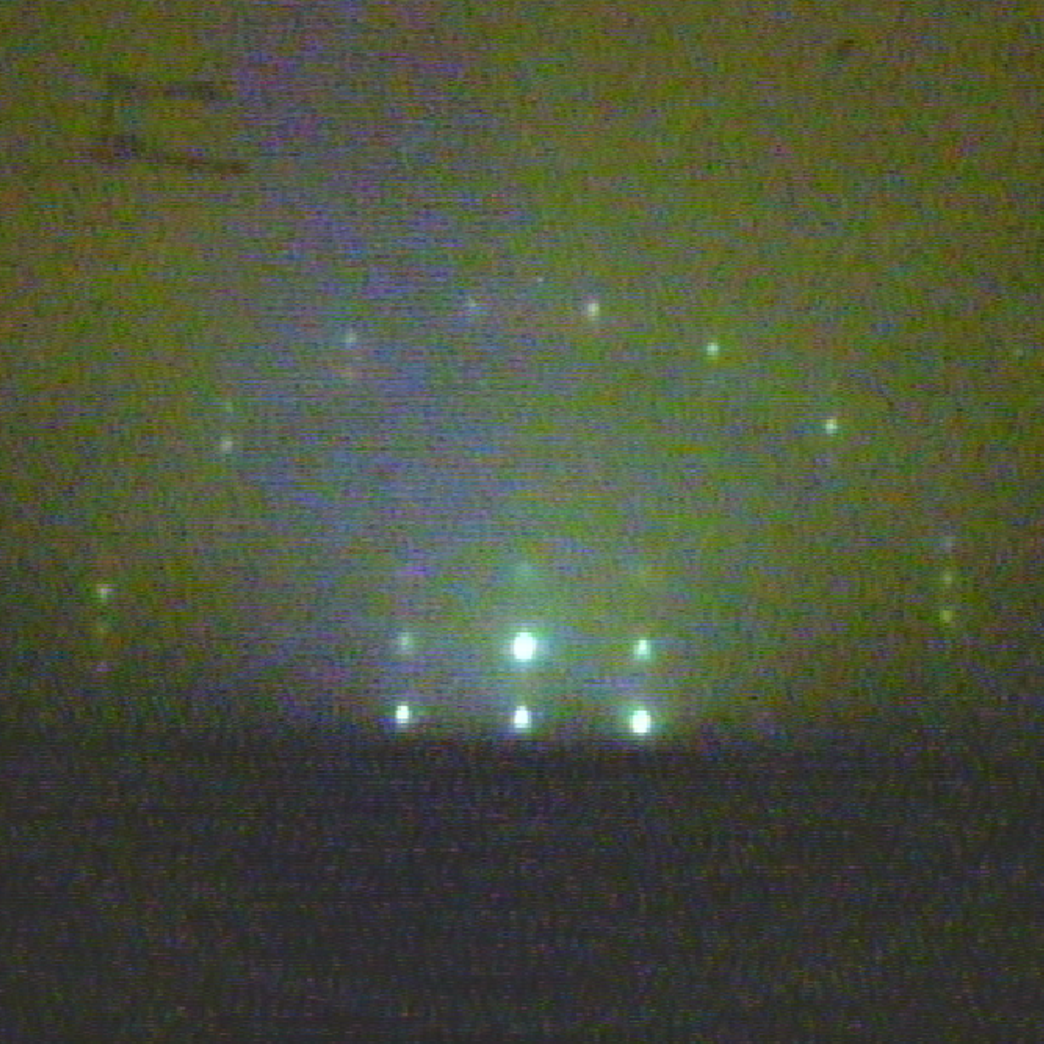
\includegraphics[width=\textwidth]{../data/edited/2_2_293deg.pdf}
        \caption{\qty{270}{\degree}}
    \end{subfigure}
    \begin{subfigure}{0.2\linewidth}
        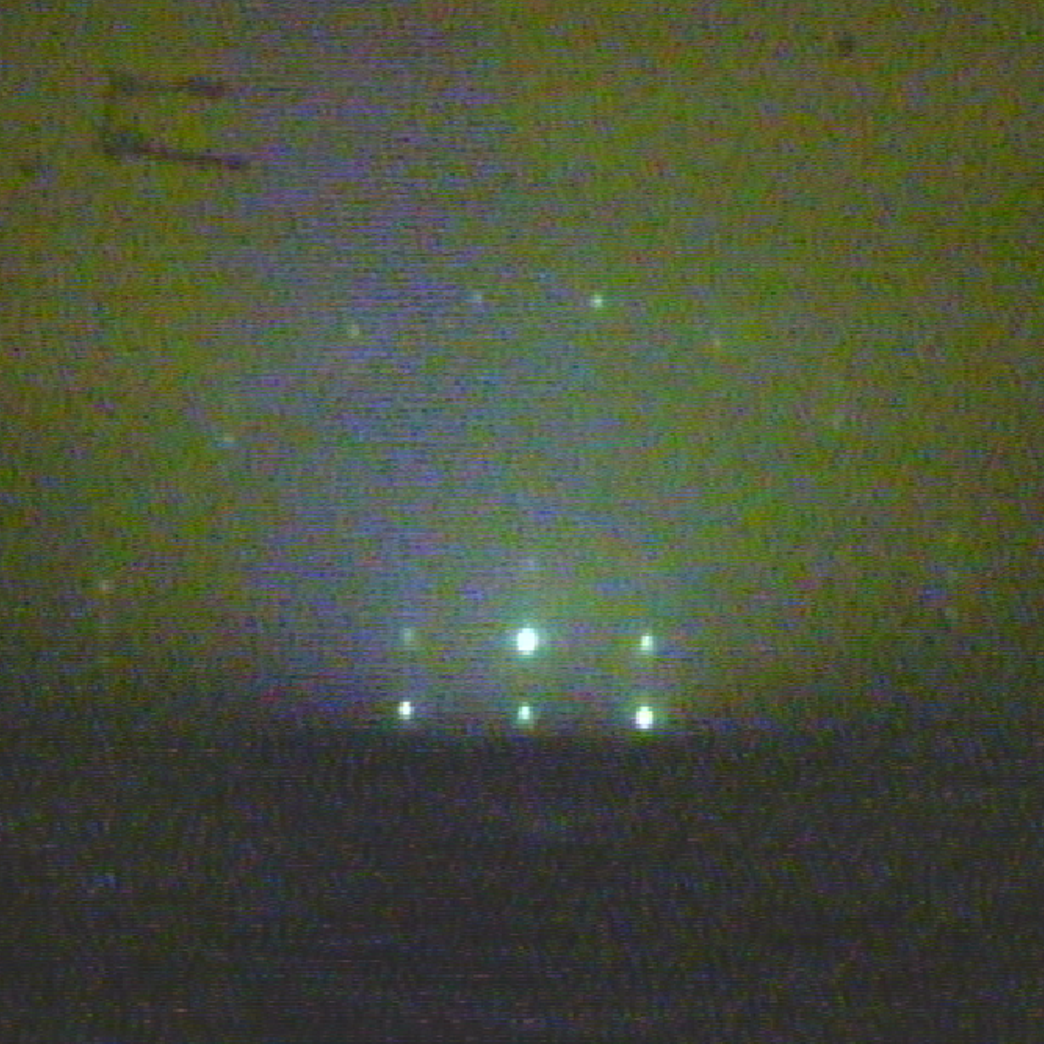
\includegraphics[width=\textwidth]{../data/edited/2_2_353deg.pdf}
        \caption{\qty{330}{\degree}}
    \end{subfigure}

    \caption{\ac{rheed} patterns of the \ce{ZnO} thin film for different azimuthal 
    angles. }
    \label{fig:rheed2}
\end{figure*}